\documentclass[]{article}
\usepackage{lmodern}
\usepackage{amssymb,amsmath}
\usepackage{ifxetex,ifluatex}
\usepackage{fixltx2e} % provides \textsubscript
\ifnum 0\ifxetex 1\fi\ifluatex 1\fi=0 % if pdftex
  \usepackage[T1]{fontenc}
  \usepackage[utf8]{inputenc}
\else % if luatex or xelatex
  \ifxetex
    \usepackage{mathspec}
  \else
    \usepackage{fontspec}
  \fi
  \defaultfontfeatures{Ligatures=TeX,Scale=MatchLowercase}
\fi
% use upquote if available, for straight quotes in verbatim environments
\IfFileExists{upquote.sty}{\usepackage{upquote}}{}
% use microtype if available
\IfFileExists{microtype.sty}{%
\usepackage{microtype}
\UseMicrotypeSet[protrusion]{basicmath} % disable protrusion for tt fonts
}{}
\usepackage[margin=1.5cm]{geometry}
\usepackage{hyperref}
\hypersetup{unicode=true,
            pdftitle={Supplementary Figures},
            pdfauthor={Pierre-Luc Germain},
            pdfborder={0 0 0},
            breaklinks=true}
\urlstyle{same}  % don't use monospace font for urls
\usepackage{natbib}
\bibliographystyle{plainnat}
\usepackage{graphicx,grffile}
\makeatletter
\def\maxwidth{\ifdim\Gin@nat@width>\linewidth\linewidth\else\Gin@nat@width\fi}
\def\maxheight{\ifdim\Gin@nat@height>\textheight\textheight\else\Gin@nat@height\fi}
\makeatother
% Scale images if necessary, so that they will not overflow the page
% margins by default, and it is still possible to overwrite the defaults
% using explicit options in \includegraphics[width, height, ...]{}
\setkeys{Gin}{width=\maxwidth,height=\maxheight,keepaspectratio}
\IfFileExists{parskip.sty}{%
\usepackage{parskip}
}{% else
\setlength{\parindent}{0pt}
\setlength{\parskip}{6pt plus 2pt minus 1pt}
}
\setlength{\emergencystretch}{3em}  % prevent overfull lines
\providecommand{\tightlist}{%
  \setlength{\itemsep}{0pt}\setlength{\parskip}{0pt}}
\setcounter{secnumdepth}{0}
% Redefines (sub)paragraphs to behave more like sections
\ifx\paragraph\undefined\else
\let\oldparagraph\paragraph
\renewcommand{\paragraph}[1]{\oldparagraph{#1}\mbox{}}
\fi
\ifx\subparagraph\undefined\else
\let\oldsubparagraph\subparagraph
\renewcommand{\subparagraph}[1]{\oldsubparagraph{#1}\mbox{}}
\fi

%%% Use protect on footnotes to avoid problems with footnotes in titles
\let\rmarkdownfootnote\footnote%
\def\footnote{\protect\rmarkdownfootnote}

%%% Change title format to be more compact
\usepackage{titling}

% Create subtitle command for use in maketitle
\providecommand{\subtitle}[1]{
  \posttitle{
    \begin{center}\large#1\end{center}
    }
}

\setlength{\droptitle}{-2em}

  \title{Supplementary Figures}
    \pretitle{\vspace{\droptitle}\centering\huge}
  \posttitle{\par}
    \author{Pierre-Luc Germain}
    \preauthor{\centering\large\emph}
  \postauthor{\par}
      \predate{\centering\large\emph}
  \postdate{\par}
    \date{12 Mai, 2019}


\begin{document}
\maketitle

{
\setcounter{tocdepth}{2}
\tableofcontents
}
\newpage

\hypertarget{supplementary-figure-1}{%
\section{Supplementary Figure 1}\label{supplementary-figure-1}}

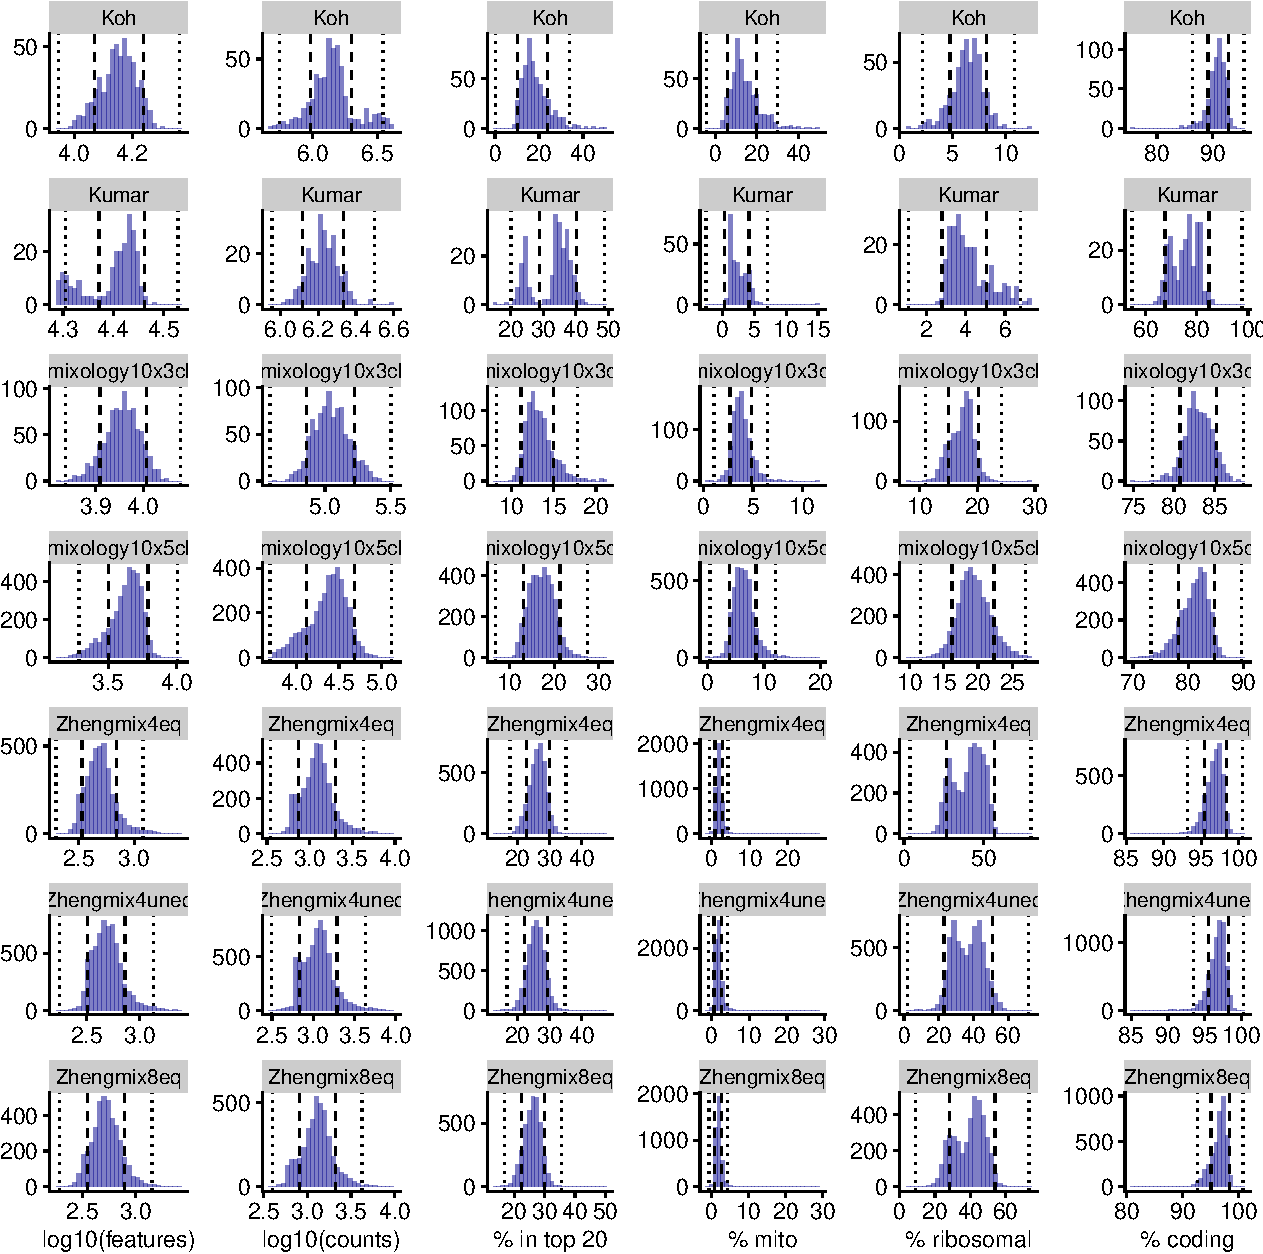
\includegraphics{supp_figures_files/figure-latex/dist_cell_properties-1.pdf}

\vfill

\hypertarget{supplementary-figure-1-1}{%
\subsubsection{Supplementary Figure 1}\label{supplementary-figure-1-1}}

Distribution across cells of various control properties in the different
datasets. The lines indicate respectively 2 and 5 median absolute
deviations (MADs).

\newpage

\hypertarget{supplementary-figure-2}{%
\section{Supplementary Figure 2}\label{supplementary-figure-2}}

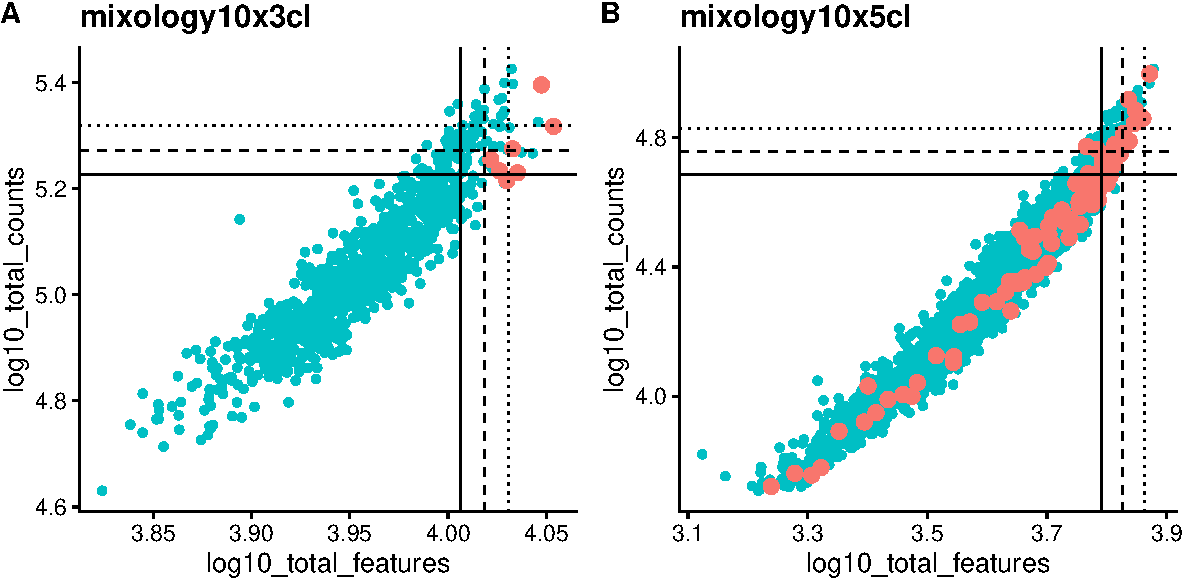
\includegraphics{supp_figures_files/figure-latex/mixology_doublet_featcount-1.pdf}

\vfill

\hypertarget{supplementary-figure-2-1}{%
\subsubsection{Supplementary Figure 2}\label{supplementary-figure-2-1}}

The total counts and total features per cell of doublets (red) versus
other cells. We used the demuxlet annotation of doublets (based on SNPs)
made available through CellBench. The lines indicate, respectively, 2,
2.5, and 3 median absolute deviations. While doublets tend to have a
higher total count and especially number of detected features, these
features alone are not always sufficient for their identification.

\newpage

\hypertarget{supplementary-figure-3}{%
\section{Supplementary Figure 3}\label{supplementary-figure-3}}

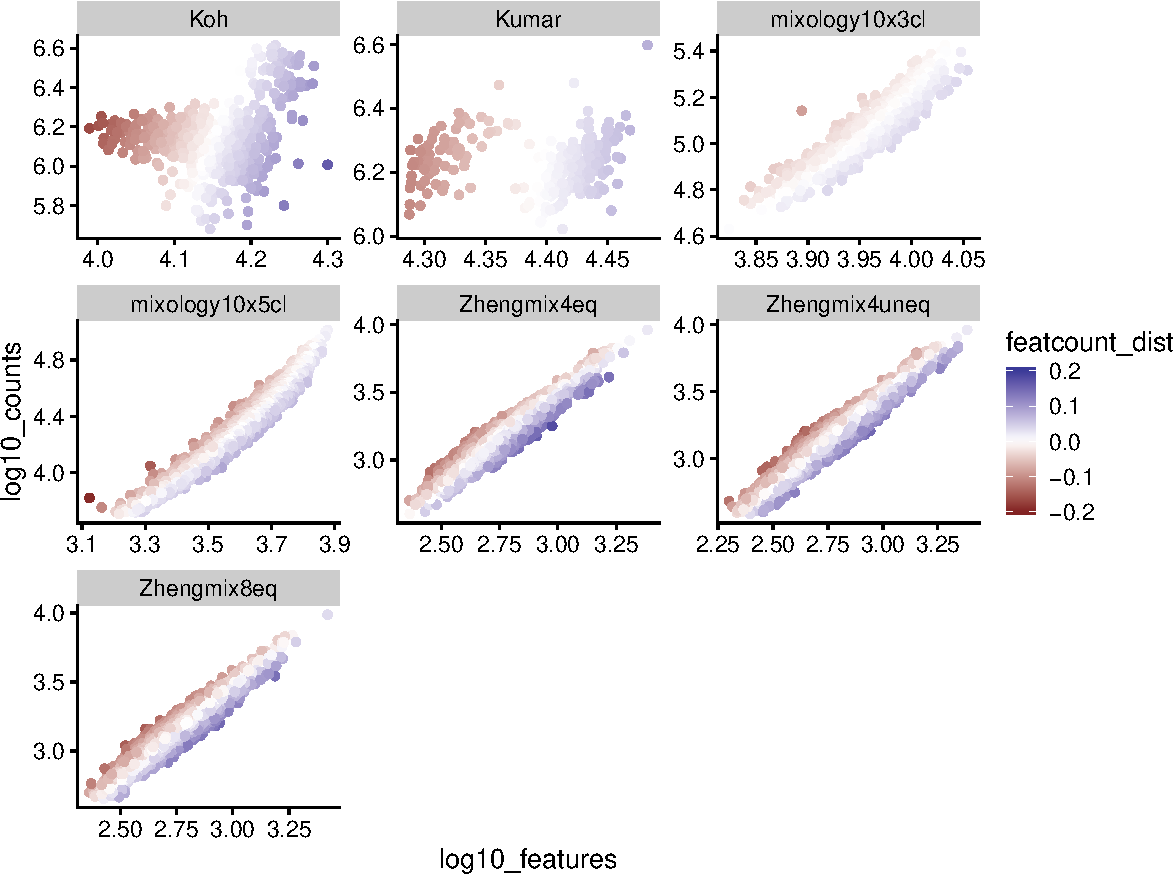
\includegraphics{supp_figures_files/figure-latex/featcount_ratio-1.pdf}

\vfill

\hypertarget{supplementary-figure-3-1}{%
\subsubsection{Supplementary Figure 3}\label{supplementary-figure-3-1}}

There is a tight relationship, in 10x datasets (i.e.~not the
\texttt{Koh} and \texttt{Kumar} datasets), between the total counts of a
cell and its number of detected features. We therefore include, among
control variables, deviation from this ratio.

\newpage

\hypertarget{supplementary-figure-4}{%
\section{Supplementary Figure 4}\label{supplementary-figure-4}}

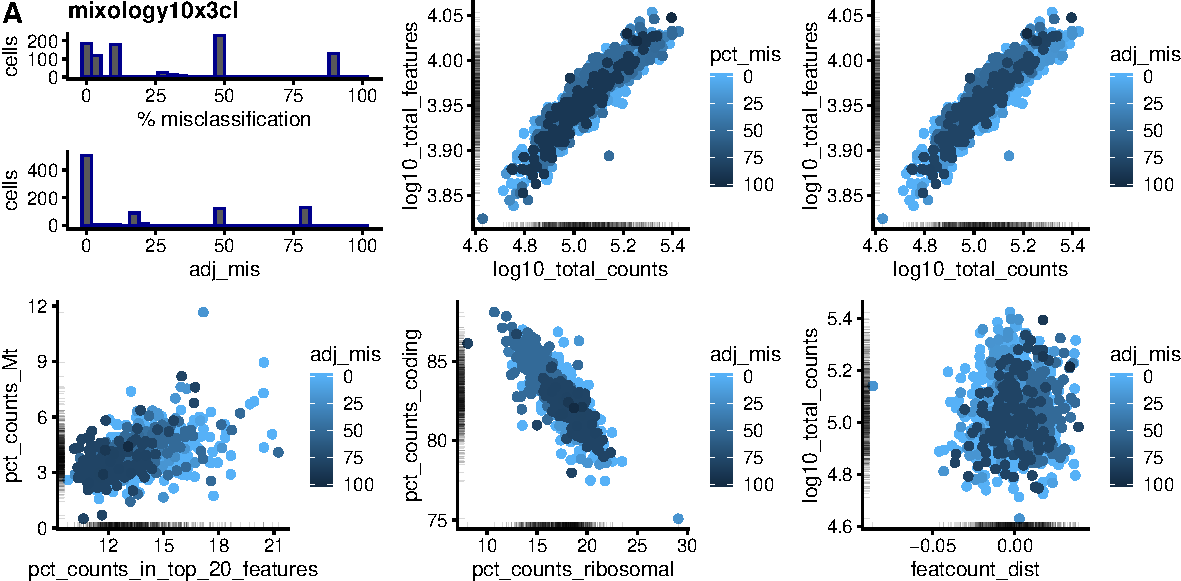
\includegraphics{supp_figures_files/figure-latex/misclass-1.pdf}
\vspace{1cm}
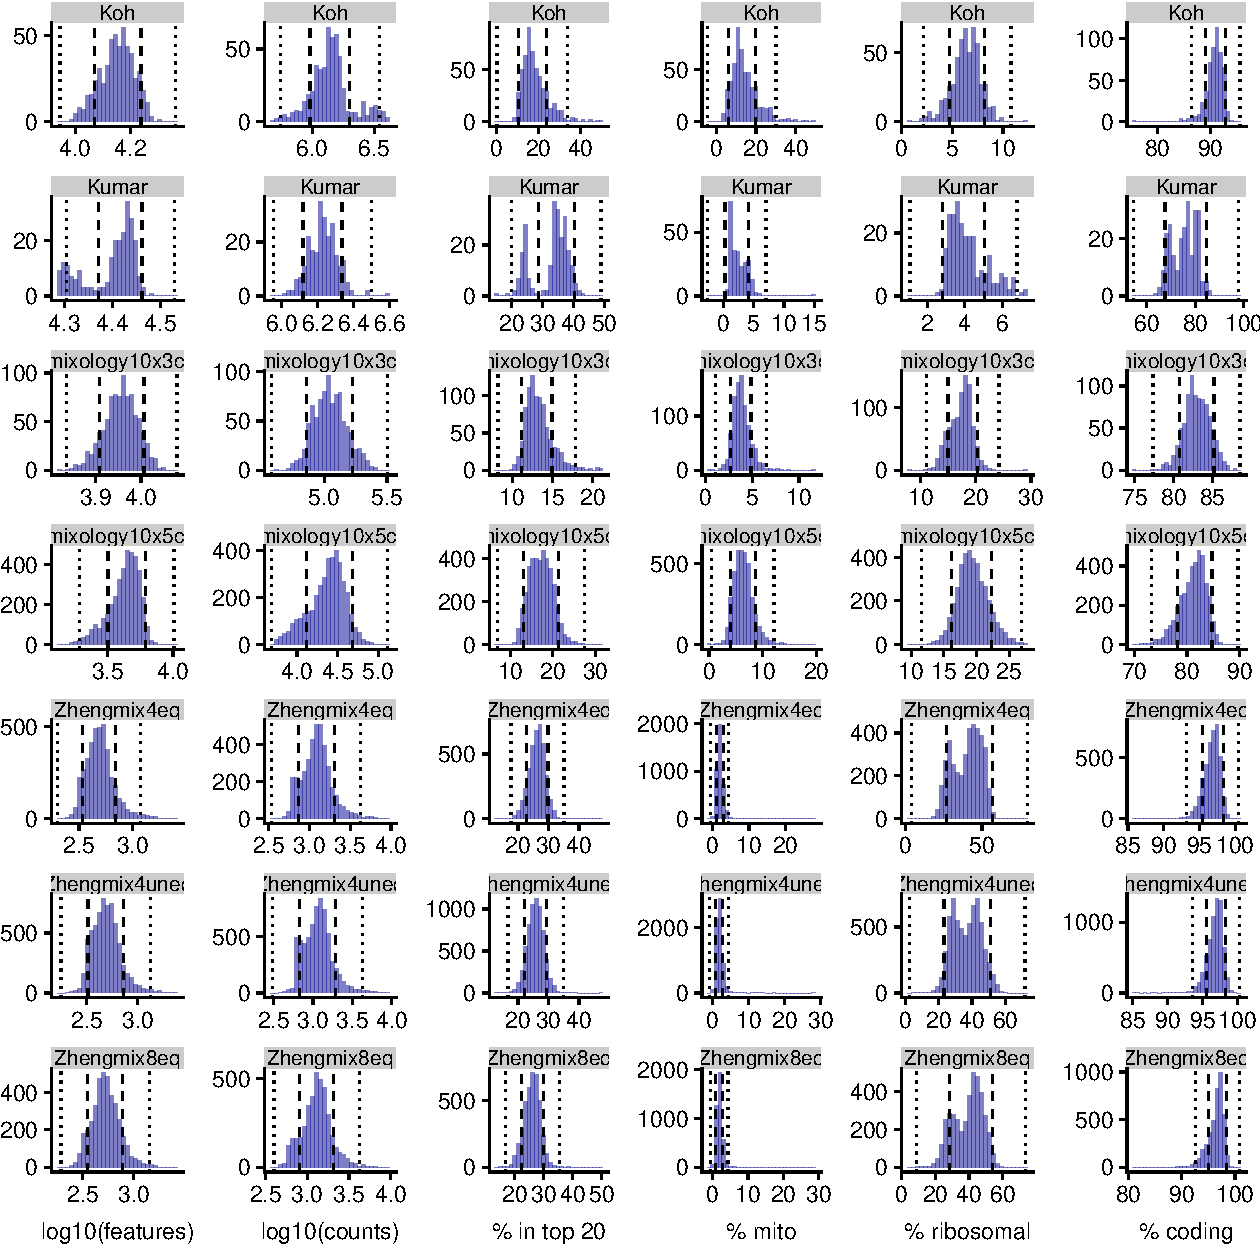
\includegraphics{supp_figures_files/figure-latex/unnamed-chunk-4-1.pdf}

\vfill

\hypertarget{supplementary-figure-4-1}{%
\subsubsection{Supplementary Figure 4}\label{supplementary-figure-4-1}}

Relationship between various cellular properties and the frequency of
cluster mis-assignment for the mixology10x3cl (A) and mixology10x5cl (B)
datasets. The percentage of misclassification refers to the frequency
with which a given cell is assigned the wrong cluster (using the
Hungarian algorithm for cluster matching) across several hundred
clustering runs with varying parameters. Since some subpopulations tend
to be more misclassified than others, the adjusted rate of
misclassification (\texttt{adj\_mis}) is substracted for the
subpopulation median misclassification rate.

\newpage

\hypertarget{supplementary-figure-5}{%
\section{Supplementary Figure 5}\label{supplementary-figure-5}}

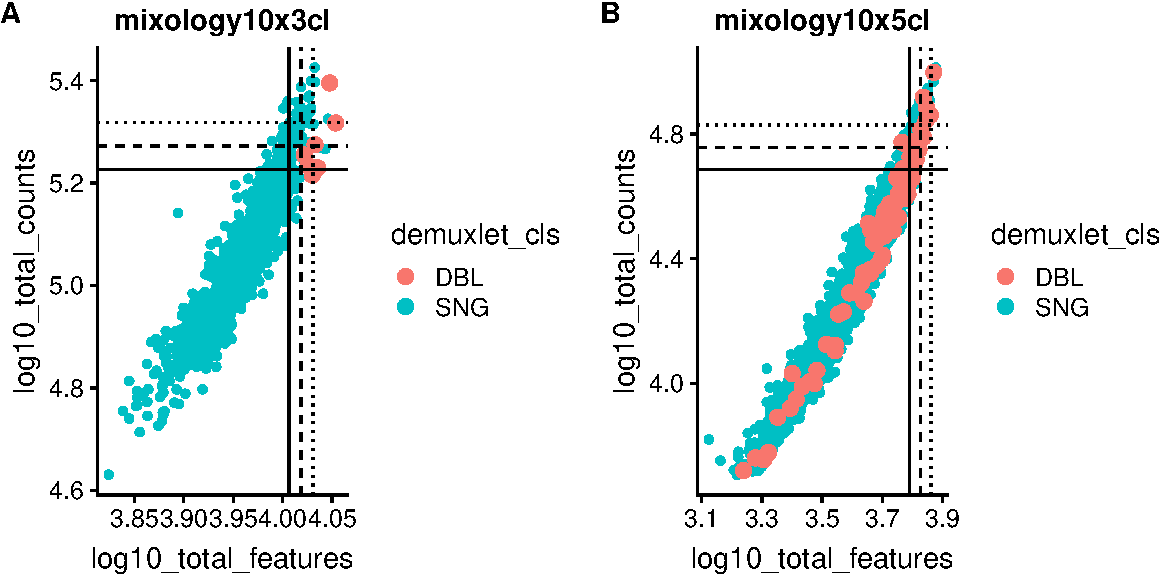
\includegraphics{supp_figures_files/figure-latex/unnamed-chunk-5-1.pdf}
\vspace{1cm}
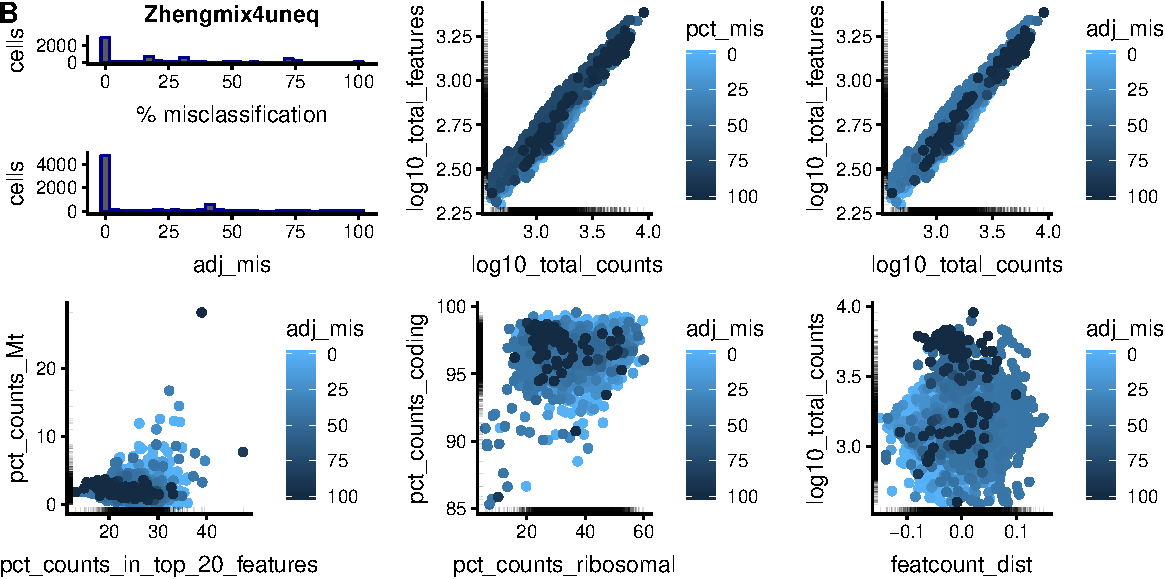
\includegraphics{supp_figures_files/figure-latex/unnamed-chunk-6-1.pdf}

\vfill

\hypertarget{supplementary-figure-5-1}{%
\subsubsection{Supplementary Figure 5}\label{supplementary-figure-5-1}}

Relationship between various cellular properties and the frequency of
cluster mis-assignment for the Zheng equal (A) or unequal (B) mixtures
of four cell types. See Supplementary Figure 4 for more information. The
only clear pattern is that cells with a high number of reads or features
tend to have a higher misclassification rate.

\newpage

\hypertarget{supplementary-figure-6}{%
\section{Supplementary Figure 6}\label{supplementary-figure-6}}

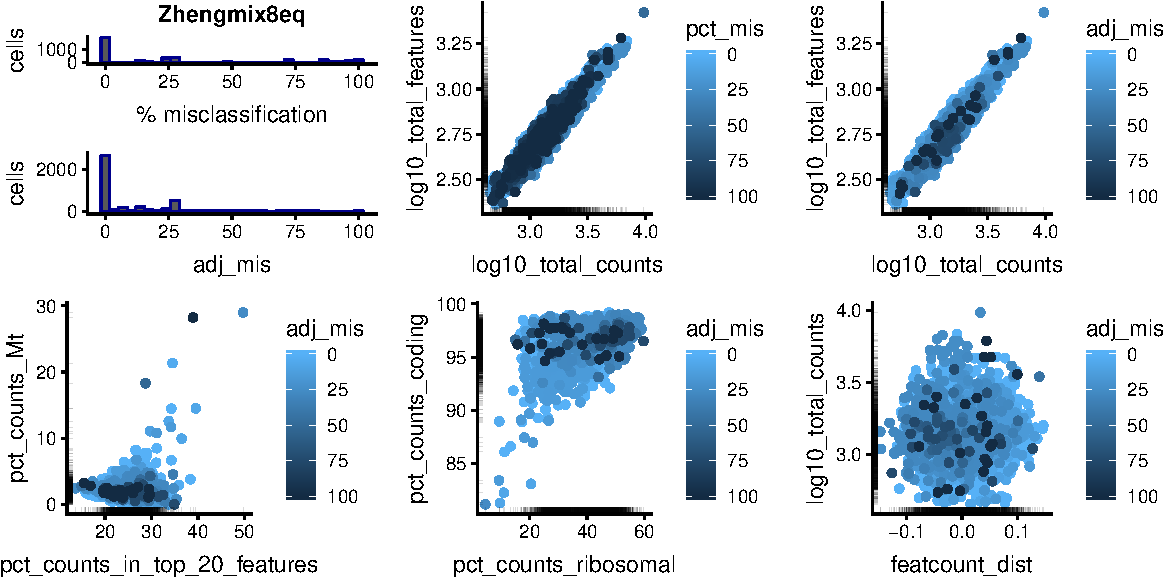
\includegraphics{supp_figures_files/figure-latex/unnamed-chunk-7-1.pdf}

\vfill

\hypertarget{supplementary-figure-6-1}{%
\subsubsection{Supplementary Figure 6}\label{supplementary-figure-6-1}}

Relationship between various cellular properties and the frequency of
cluster mis-assignment for the Zheng mixture of 8 cell types. See
Supplementary Figure 4 for more information.

\newpage

\bibliography{../bmc\_article.bib}


\end{document}
